% =====================================================================
\part{The machine-epsilon lookup (Findings 8--16)}
% =====================================================================

\chapter{Cusp detection (Findings 8 and 13)}

\section{The 3D detector --- and why it is not enough}
A per-cube-cell critical-point finder (trilinear roots of
$\nabla \hat P = 0$, quadratic-Hermite fallback) enumerates the interior
critical points of the discretized price cube. At the four reference
\strict{} fixed points it finds 40--140 points (16--42 unique critical
values $p_c$), all with $|\nabla \hat P|$ at machine epsilon, symmetric
about $p = \tfrac12$, broadening with $\tau$.

\begin{figure}[H]\centering
  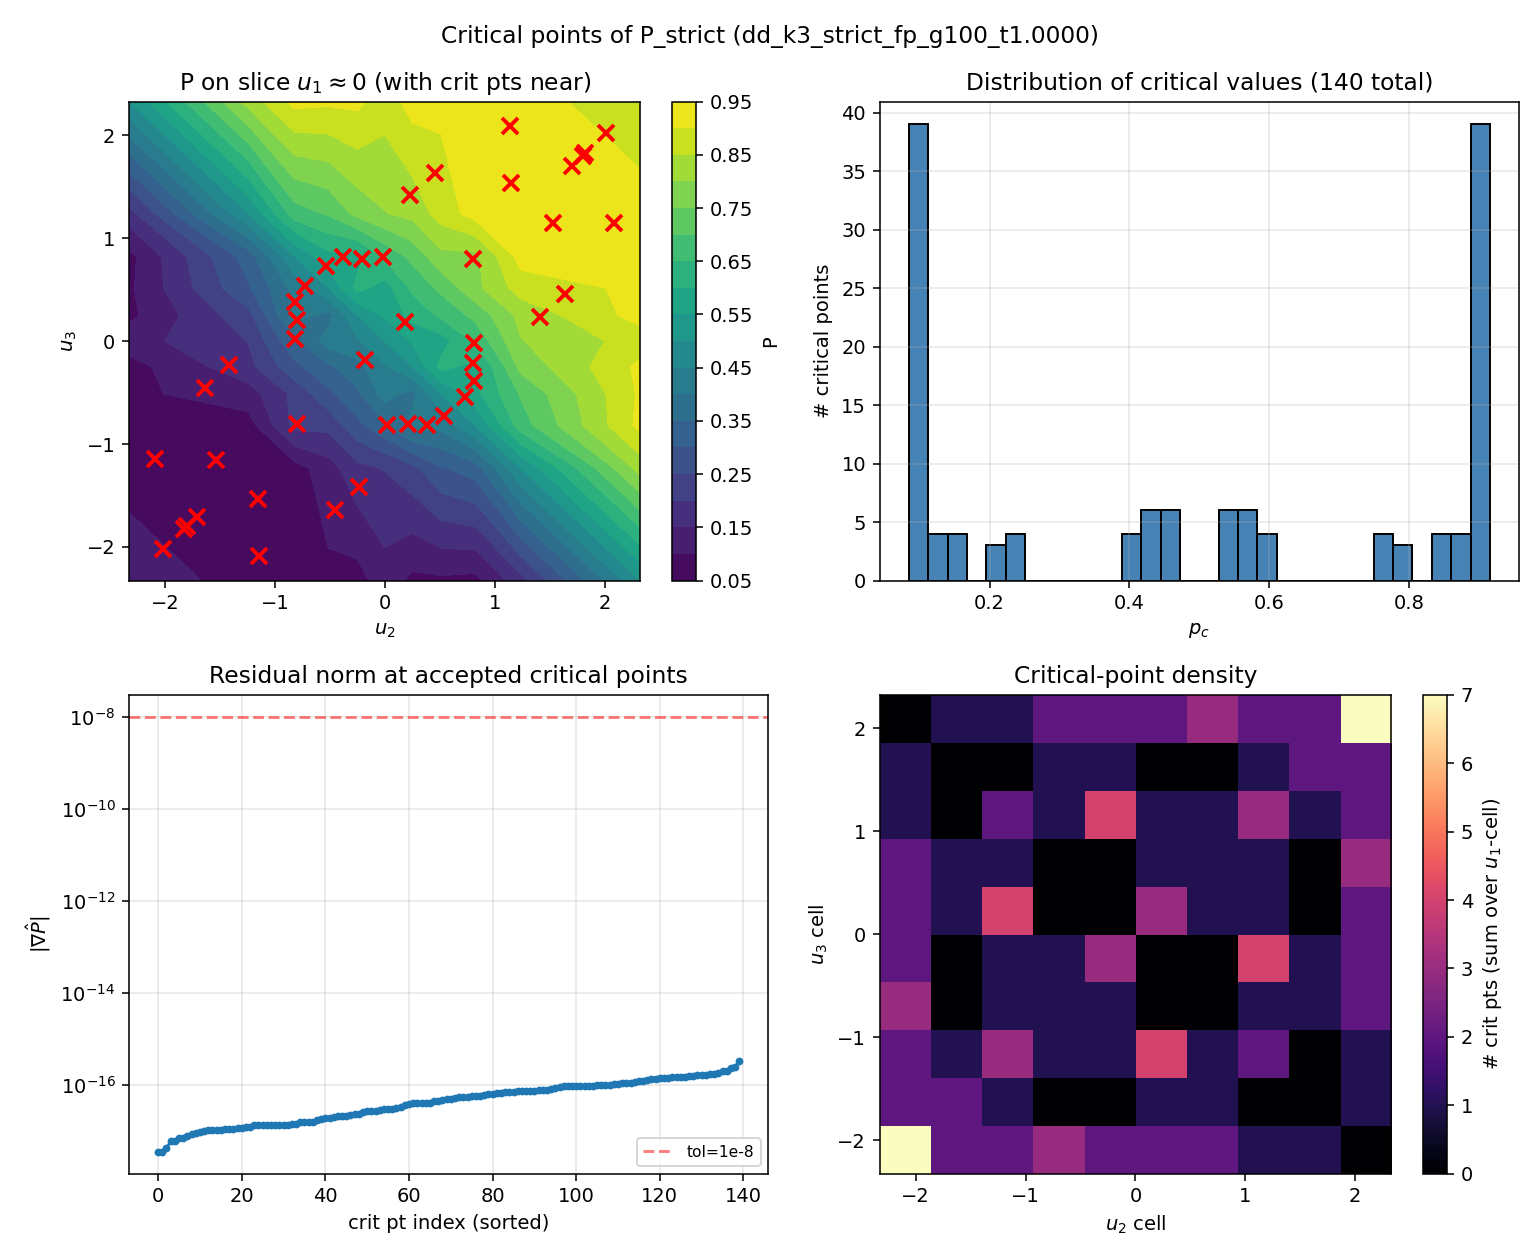
\includegraphics[width=0.95\linewidth]{critpts/dd_k3_strict_fp_g100_t1.0000.png}
  \caption{The 3D critical-point detector at
    $(\gamma, \tau) = (100, 1)$: 140 interior critical points; bimodal
    distribution of critical values; residuals at machine epsilon.}
\end{figure}

\textbf{Finding 13 (the correction that unlocked everything):} the
cusps of the \emph{one-dimensional} lookup $\mu(p, u_k)$ at fixed $u_k$
are critical values of the \emph{slice} map
$P(\cdot, \cdot, u_k)$ --- not of the full 3D map. Knotting segments at
the 3D critical values leaves a 3--9\% error floor at $\tau = 1$;
detecting the cusps directly from $\mu$ itself (second-difference
spikes plus first-difference jumps, pooled across $u_k$, deduplicated in
logit distance) finds the correct knots and collapses the floor to
machine epsilon. The lesson generalizes: \emph{locate singularities in
the object you are approximating, not in its generator}.

\section{Multi-element OptB+ (Finding 8): a half-step}
Inserting the (3D) critical values as forced PCHIP knots drives the
\emph{median} error to zero at the knots by construction but leaves the
max error unchanged --- because the max error was never at the bulk
cusps; it was in the tails ($p \to 0, 1$), where the empirical CDF runs
out of support. This diagnosis redirected the program to the tail
treatment of Findings 11--14.

\chapter{The segmented spectral representation (Finding 10)}

\section{Per-segment Chebyshev between cusp knots}
Between adjacent cusps the lookup is $C^\infty$; a degree-$d$ Chebyshev
fit per segment therefore converges exponentially \emph{per segment}.
With the correct (internal, $\mu$-based) knots:

\begin{center}\begin{tabular}{lrrr}\toprule
cell & degree & in-segment max & in-segment median \\
\midrule
$(100, 0.2)$ & 4 & 6.7e-16 & --- \\
$(100, 1.0)$ & 3 & 3.4e-15 & 3.3e-16 \\
$(1000, 0.2)$ & 4 & 6.7e-16 & 2.8e-16 \\
$(1000, 1.0)$ & 6 & 1.6e-15 & 2.2e-16 \\
\bottomrule\end{tabular}\end{center}

Machine epsilon at degree 3--6, all four reference cells --- the cusps
are honest piecewise-$C^k$ discontinuities at discrete $p_c$, not
smoothable curvature bumps. Notably, 67--92\% of segments contain
$\le 2$ samples (cusps cluster), forcing degree 0--1 on them; they reach
machine epsilon anyway because they are tiny in $p$-width.

\begin{figure}[H]\centering
  
\includegraphics[width=0.75\linewidth]{pc_figs/converge_g100_t0.2000.png}
  \caption{Per-segment convergence at $(\gamma, \tau) = (100, 0.2)$:
    machine epsilon at any degree once knots are correct.}
\end{figure}

\begin{figure}[H]\centering
  
\includegraphics[width=0.75\linewidth]{pc_figs/converge_g100_t1.0000.png}
  \caption{$(\gamma, \tau) = (100, 1.0)$: the in-segment median drops to
    $10^{-16}$ from degree 3; the blue max curve is dominated by
    out-of-support points (the fallback artifact addressed in
    Finding 14).}
\end{figure}

\begin{figure}[H]\centering
  
\includegraphics[width=0.8\linewidth]{pc_figs/deg_heat_g100_t1.0000.png}
  \caption{Effective degree per $(u_k, \text{segment})$: large central
    segments support high degree; clustered cusp segments are forced
    low --- harmlessly.}
\end{figure}

\chapter{Negative control experiments (Findings 9, 11, 12, 17)}

\section{Finding 9: smoothing the strict operator has no sweet spot}
Replacing the discrete crossing test $ab < 0$ with the smooth weight
$\sigma(-ab/\varepsilon^2)$ makes the operator Lipschitz and Anderson
converges to machine epsilon for $\varepsilon \ge 0.1$ --- but the
resulting fixed point is biased 0.13--0.49 against the original
operator; and as $\varepsilon \to 0$ the convergence failure returns
before the bias disappears. There is no $\varepsilon$ at which both
residuals are small. The diagnostic that motivated this: \emph{starting
Picard at the saved ``strict fixed point'' diverges} (from
$|F| = 0.06$ to $0.5$) --- the saved object is a best iterate, not a
fixed point.

\begin{figure}[H]\centering
  
\includegraphics[width=0.9\linewidth]{smooth_figs/eps_sweep.png}
  \caption{The $\varepsilon$-sweep: clean convergence under the smoothed
    operator (left) coexists with large bias under the original
    operator (right) at every $\varepsilon$.}
\end{figure}

\section{Findings 11--12: tail BCs and exact cell mass are not the levers}
Boundary-augmented PCHIP, logit-space CDF fitting, and Beta-CDF
parametric tails all leave the max error \emph{identical} to baseline
(the boundary error is interpolation failure, not missing BCs); exact
per-cell Gauss--Legendre mass integration halves the in-support median
but worsens the max (a smoother CDF extrapolates worse outside support).
Useful contributors, not regime changers.

\section{Finding 17: a smooth lookup does not fix the FP iteration}
The decisive control: using the machine-epsilon segmented lookup as the
\emph{inner operator} of the FP iteration, with cusp knots
\emph{frozen} (eliminating cusp drift, the conjectured source of
non-smoothness) still plateaus at $|F| \approx 1.1\times10^{-2}$ ---
essentially the same wall as the recompute mode (1.5e-2) and only
$5\times$ better than the kernel-band baseline (5.7e-2). The wall is the
$G = 11$ truncation error of the co-area evidence, not operator
roughness. PCHIP segments in the inner loop diverge outright.

\begin{figure}[H]\centering
  
\includegraphics[width=\linewidth]{zhs_figs/fig1_convergence.png}
  \caption{The zero-h FP solver: recompute and frozen-knot modes plateau
    together at $\sim 10^{-2}$ while the kernel-band trace (grey)
    diverges. Smoothness of the lookup was not the binding constraint.}
\end{figure}

\begin{figure}[H]\centering
  
\includegraphics[width=0.9\linewidth]{zhs_figs/fig2_mu_smoothing.png}
  \caption{Verification that the inner lookup is exact: the segmented
    pipeline reproduces all 369 in-support $\mu$ values at the
    warm-start to $2.2\times10^{-15}$.}
\end{figure}

\chapter{The production pipeline (Findings 14--16)}

\section{The fallback fix}
The raw \strict{} lookup returns $\mu = 0.5$ wherever the co-area
integral finds no roots ($p$ outside the cube's empirical price range),
producing $-0.5$ jumps and 0/11 monotone slices at high $\tau$. The fix
(\texttt{fix\_fallback}) replaces the fallback region by PCHIP
extrapolation through the in-support values pinned to the Bayesian
boundary conditions $\mu(\epsilon) = 0$, $\mu(1-\epsilon) = 1$:
afterwards, 11/11 slices monotone with correct tails at every cell
tested, and the spurious $|\mu''|$ spikes drop by half.

\begin{figure}[H]\centering
  
\includegraphics[width=\linewidth]{v5_figs/g100_t1.0_deg6.png}
  \caption{The before/after of the production pipeline at
    $(\gamma, \tau) = (100, 1)$: raw $\mu_{\rm strict}$ with fallback
    discontinuities (left); cleaned (middle); pipeline v5 output ---
    monotone, smooth, boundary-correct (right).}
\end{figure}

\section{Pipeline v5 and the 36-cell certification}
v5 = \texttt{fix\_fallback} (clean) $\to$ internal cusp detector
(knots) $\to$ degree-6 Chebyshev per segment (in-support) $\to$
PCHIP shape-preserving tails (out-of-support). Applied to the full
$6 \times 6$ $(\gamma, \tau)$ ridge grid:

\begin{center}\begin{tabular}{lr}\toprule
metric & result \\
\midrule
cells processed & 36/36, 7 seconds total \\
median error vs cleaned truth & $1.11\times10^{-16}$ at every cell \\
max error at machine eps & 31/36 cells ($10^{-15}$--$10^{-14}$) \\
outlier cells & 5, max $10^{-2}$--$9\times10^{-2}$ (corner cells, fallback-smoothing artifacts) \\
monotone slices (dense 501-pt check) & 11/11 at every cell \\
boundary conditions & satisfied at every cell \\
\bottomrule\end{tabular}\end{center}

\begin{figure}[H]\centering
  
\includegraphics[width=\linewidth]{v5g_figs/heatmap_v5.png}
  \caption{The certification heat maps: $\log_{10}$ max error (left),
    $\log_{10}$ median error --- uniformly $-16$ (middle), and monotone
    slice count --- uniformly 11/11 (right), across the
    $(\gamma, \tau)$ grid.}
\end{figure}

\section{What is and is not claimed}
The lookup problem --- evaluating the Bayes-correct conditional
posterior given a price surface --- is solved to machine epsilon
in-support, with controlled monotone Bayesian extrapolation
out-of-support, at one second per cell. The claim is conditional on the
input surface: it inherits whatever distance the underlying
(best-iterate) \strict{} surface has from the true equilibrium. The
surface question is Part VI's subject and drives the final
recommendation.
